\chapter{Læsevejledning}
Dette bachelorprojekt består af to sideløbende delprojekter: 

\begin{itemize}
	\item Delstudie 1 - Udviklingsprojekt: Udvikling af en prototype af et detekteringssystem til anvendelse under proceduren BF-ViV og eksperimentelle forsøg 
	\item Delstudie 2 - Forskningsprojekt: Undersøge hvorledes det nødvendige fraktureringstryk påvirkes ved forskellige kalcificeringsgrader af aortarodens annulus  
\end{itemize}

Den overordnede projektrapport er derfor inddelt i to rapporter. Rapporten for udviklingsprojektet ses fra Kapitel \ref{detekteringssystem} og rapporten for forskningsprojektet ses fra Kapitel \ref{forskning}.  


På Figur \ref{flow1} vises de forskellige forstudier, der er blevet udført for henholdsvis Delstudie 1 og 2 vist, samt deres indbyrdes interaktioner. 

\begin{figure}[H]
	\centering
	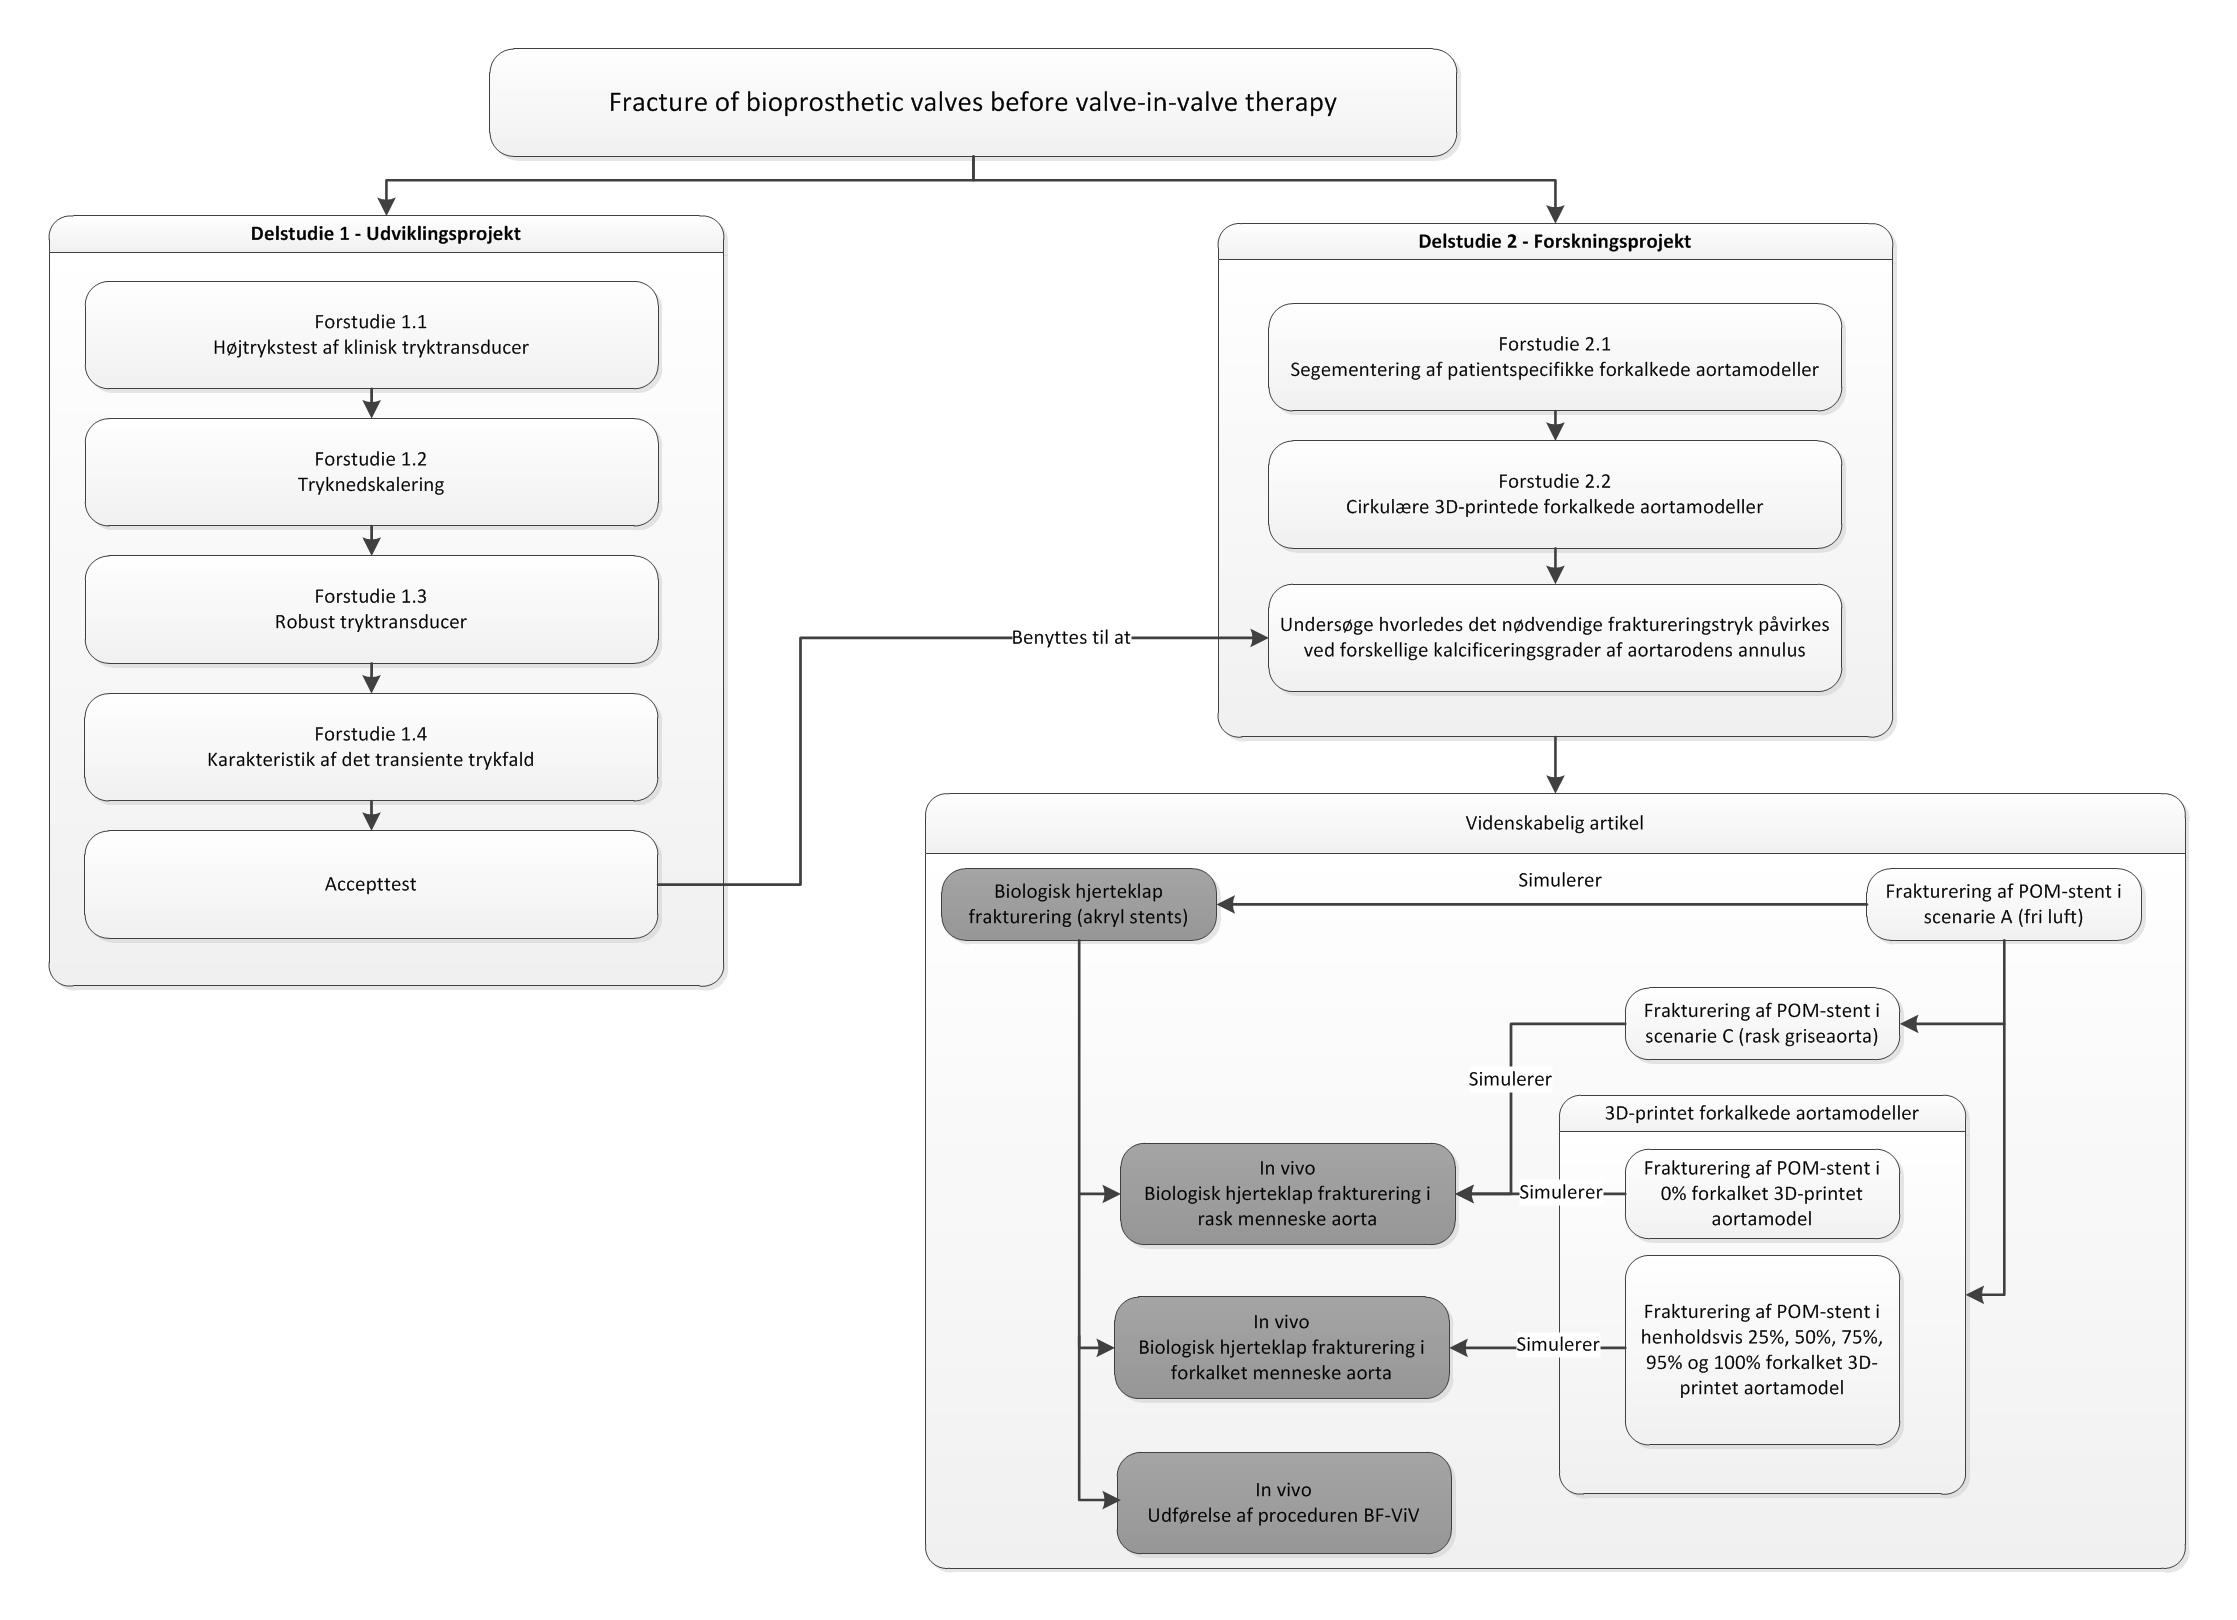
\includegraphics[width=1\textwidth]{Figure/flowchart}
	\caption{Illustration af de forskellige forstudier, der er blevet udført gennem udarbejdelsen af dette bachelorprojekt. Boksen "Videnskabelig artikel"\ illustrerer de eksperimentelle forsøg, der danner grundlag for indholdet af den videnskabelige artikel. De mørkegrå bokse repræsenterer forsøg, som ikke er blevet udført}
    \label{flow1}
\end{figure}

Udviklingsprojektet består af systemkrav, som indledningsvist er defineret. Herefter er arkitekturen, design, implementering og test udarbejdet. Udviklingsprocessen samt forstudierne er dokumenteret i Projektdokumentationen.

Forskningsprojektet er opbygget på baggrund af den videnskabelige rapportstruktur IMRAD (Introduction, Methods, Results, and Discussion). Forstudierne er dokumenteret i Projektdokumentationen.       

Den videnskabelige artikel er ikke et produkt i dette bachelorprojekt. Forsøgsresultater fra Forstudie 1.4 (Scenarie A og C) samt fra Delstudie 2, skal anvendes til publicering af den videnskabelige artikel, der præsenterer resultaterne for den samlede forskning omhandlende den nye procedure indenfor interventionel kardiologi, BF-ViV. 

Projektrapporten præsenterer det samlede resultat af bachelorprojektet. Gennem Projektrapporten er der henvist til Projektetdokumentationen samt til bilag, hvor ydereligere detaljer samt argumentation for det skrevne er dokumenteret. En henvisning til Projektdokumentationen ser således ud: Se dokumentation Kapitel/afsnit x. En henvisning til projektets bilag ser således ud: Se Bilag x.  
    

